\section{Fast--slow EESM reduction and a reproducible transition experiment}
\label{sec:fast-slow-experiment}

Define representative electrical time constants
\[
 \gls{sym:taus}=\sqrt{\frac{L_{\mathrm d}}{R_s}
                         \frac{L_{\mathrm q}}{R_s}},
 \qquad
 \gls{sym:tauexc}=\frac{L_{\mathrm f}}{R_{\mathrm{exc}}},
 \qquad
 \gls{sym:epsilon}=\frac{\tau_s}{\tau_f}.
 \tag{32.1}
\]
When \(\varepsilon\ll1\), stator currents are fast and field current is slow.
After rescaling time by \(\tau_f\), singular-perturbation reasoning suggests a
fast layer in \((i_d,i_q)\) followed by slow motion of \(i_f\).  This is a
model property, not a universal EESM fact: coupling, converter ratios, and
back-EMF may destroy the separation even when \(L_f/R_f\) is large.

For a fixed slow field current and requested torque define the conditional
steady optimum
\[
 \mathcal I^\star(i_f,M_{\mathrm{ref}})=
 \arg\min_{i_d,i_q}P_{\mathrm{Cu}}
 \quad\text{s.t.}\quad M=M_{\mathrm{ref}}
 \text{ and instantaneous constraints}.
 \tag{32.2}
\]
If the fast subsystem is stable and its constraint margin is uniform, the
stator state can track this moving optimum manifold while \(i_f\) evolves.
The three-state problem then reduces approximately to a scalar scheduling
problem for \(i_f\), with the static inner solver from Part~I reused online.

\begin{figure}[tb]
\centering
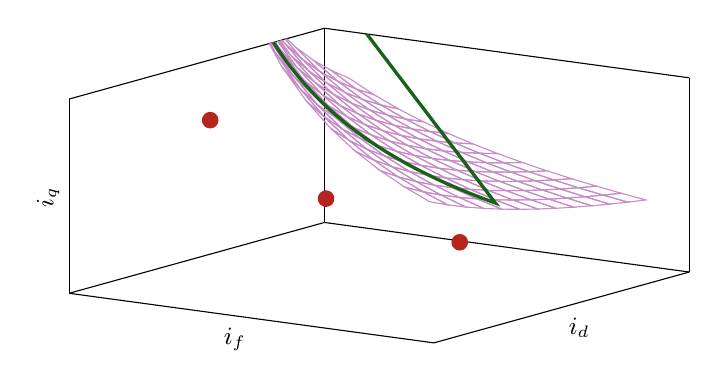
\begin{tikzpicture}[font=\small]
 \begin{axis}[width=.78\linewidth,height=.46\linewidth,view={35}{24},
  xlabel={$i_f$},ylabel={$i_d$},zlabel={$i_q$},ticks=none,
  xmin=0,xmax=2.3,ymin=-.4,ymax=2.2,zmin=0,zmax=2.4]
  \addplot3[mesh,draw=Purple!45,domain=.28:2.15,y domain=-.2:2.0,samples=13,samples y=13]
   ({x},{y},{1.15/(.25*y+.35*x)});
  \addplot3[ForestGreen!70!black,very thick,domain=.35:2.05,samples=80]
   ({x},{.22+.20*x},{1.15/(.25*(.22+.20*x)+.35*x)});
  \addplot3[only marks,mark=*,BrickRed,mark size=2.8pt]
   coordinates {(.45,.31,2.02)(1.1,.44,1.18)(1.85,.59,.79)};
 \end{axis}
\end{tikzpicture}
\caption{Moving optimum manifold.  The translucent surface is a constant
torque set; the dark curve represents the conditional minimum-loss stator
allocation as the slow field current changes.  Fast currents can track this
curve only when time-scale separation and voltage margin are adequate.}
\label{fig:moving-manifold}
\end{figure}



\subsection{Declared toy model and search family}

The reproducible script \texttt{validation/verify\_dynamics.py} uses
\[
 \matr L=\begin{bmatrix}.42&0&.12\\0&.24&0\\.12&0&1.05\end{bmatrix},
 \quad
 \matr R_e=\operatorname{diag}(.16,.16,.12),
 \quad \omega_e=.75,
 \tag{32.3}
\]
with \(U_s=1.30\), \(U_f=.32\), and \(k_T=3\) in a normalized unit system.
The inductance eigenvalues are \(0.2400,0.3979,1.0721\), so reciprocity and
positive magnetic energy are satisfied.  The time-scale ratio is
\(\varepsilon=0.2268\) with \(\tau_s=1.9843\) and \(\tau_f=8.7500\).
The step is
\[
 \vect i_A=(.05,.45,.55)^{\mathsf T},\quad
 \vect i_B=(.35,1.25,1.10)^{\mathsf T},\quad
 M_A=.10125,\quad M_B=.73125.
 \tag{32.4}
\]

Every candidate is a piecewise-linear current curve.  For each segment the
minimum feasible duration is found from the exact affine voltage along that
segment.  Convexity makes endpoint voltage checks sufficient.  The two
numerically optimized paths use two internal waypoints, deterministic random
coordinate refinement, monotonic torque, and exact stator-circle and field
voltage checks.  They are optima within that declared waypoint family, not a
proof of the global continuous-time optimum.

\begin{table}[tb]
\centering
\caption{Quantitative A-to-B comparison for the normalized linear EESM toy
case.  All paths reach unit voltage utilization within numerical tolerance.}
\label{tab:dynamic-results}
\small
\begin{tabularx}{\linewidth}{@{}lrrX@{}}
\toprule
Path & transition time & copper energy & relative interpretation\\
\midrule
Straight interpolation & 3.2633 & 0.7063 & Euclidean baseline\\
Stator first & 3.4842 & 1.6680 & rapid torque-surface hypothesis\\
Excitation first & 3.3019 & 0.4247 & slow-axis-first baseline\\
Metric-derived two-stage & 3.3876 & 1.4883 & natural-gradient target point\\
Time-oriented waypoint path & \textbf{2.7489} & 1.0458 & shortest in tested family\\
Energy-oriented waypoint path & 3.0164 & \textbf{0.3504} & \(t_f\leq1.55t_{\min}\)\\
\bottomrule
\end{tabularx}
\end{table}

The result rejects a simplistic interpretation of the fast--slow hypothesis.
Although the field time constant is 4.41 times the representative stator time
constant, the naive stator-first path is slowest and most dissipative here.
Its rapid torque acquisition demands high \(i_q\), which raises copper loss
and consumes stator voltage.  Coordinated motion is 15.8\% faster than the
straight path.  The energy-oriented path is 9.7\% slower than the tested
time-oriented path but uses 66.5\% less copper energy.  Fast--slow structure
suggests good coordinates; it does not determine the optimum by itself.

\begin{figure}[p]
\centering
\begin{tikzpicture}
\begin{groupplot}[
 group style={group size=2 by 3,horizontal sep=1.15cm,vertical sep=1.15cm},
 width=.46\linewidth,height=.25\linewidth,grid=both,
 tick label style={font=\scriptsize},label style={font=\scriptsize},
 legend style={font=\scriptsize,draw=none,fill=none}]
\nextgroupplot[ylabel={$i_d$},xlabel={$t$}]
 \addplot[gray,dashed] table[x index=0,y index=1]{figures/data/dynamic_straight.dat};
 \addplot[BrickRed,thick] table[x index=0,y index=1]{figures/data/dynamic_time.dat};
 \addplot[ForestGreen!70!black,thick] table[x index=0,y index=1]{figures/data/dynamic_energy.dat};
\nextgroupplot[ylabel={$i_q$},xlabel={$t$},legend to name=dynlegend]
 \addplot[gray,dashed] table[x index=0,y index=2]{figures/data/dynamic_straight.dat};
 \addlegendentry{straight}
 \addplot[BrickRed,thick] table[x index=0,y index=2]{figures/data/dynamic_time.dat};
 \addlegendentry{time-oriented}
 \addplot[ForestGreen!70!black,thick] table[x index=0,y index=2]{figures/data/dynamic_energy.dat};
 \addlegendentry{energy-oriented}
\nextgroupplot[ylabel={$i_f$},xlabel={$t$}]
 \addplot[gray,dashed] table[x index=0,y index=3]{figures/data/dynamic_straight.dat};
 \addplot[BrickRed,thick] table[x index=0,y index=3]{figures/data/dynamic_time.dat};
 \addplot[ForestGreen!70!black,thick] table[x index=0,y index=3]{figures/data/dynamic_energy.dat};
\nextgroupplot[ylabel={$M$},xlabel={$t$}]
 \addplot[gray,dashed] table[x index=0,y index=4]{figures/data/dynamic_straight.dat};
 \addplot[BrickRed,thick] table[x index=0,y index=4]{figures/data/dynamic_time.dat};
 \addplot[ForestGreen!70!black,thick] table[x index=0,y index=4]{figures/data/dynamic_energy.dat};
\nextgroupplot[ylabel={$P_{\rm Cu}$},xlabel={$t$}]
 \addplot[gray,dashed] table[x index=0,y index=5]{figures/data/dynamic_straight.dat};
 \addplot[BrickRed,thick] table[x index=0,y index=5]{figures/data/dynamic_time.dat};
 \addplot[ForestGreen!70!black,thick] table[x index=0,y index=5]{figures/data/dynamic_energy.dat};
\nextgroupplot[ylabel={voltage utilization},xlabel={$t$},ymax=1.08]
 \addplot[gray,dashed] table[x index=0,y index=6]{figures/data/dynamic_straight.dat};
 \addplot[BrickRed,thick] table[x index=0,y index=6]{figures/data/dynamic_time.dat};
 \addplot[ForestGreen!70!black,thick] table[x index=0,y index=6]{figures/data/dynamic_energy.dat};
 \addplot[black,dotted] coordinates {(0,1)(4,1)};
\end{groupplot}
\node at ($(current bounding box.south)+(0,-6mm)$) {\pgfplotslegendfromname{dynlegend}};
\end{tikzpicture}
\caption{Currents, torque, copper power, and exact converter utilization in
the A-to-B toy experiment.  Different paths reach the same endpoint but use
the voltage and loss budgets in visibly different ways.}
\label{fig:dynamic-profiles}
\end{figure}

\begin{figure}[tb]
\centering
\begin{tikzpicture}
 \begin{axis}[name=traj,width=.54\linewidth,height=.48\linewidth,view={42}{24},
  xlabel={$i_d$},ylabel={$i_q$},zlabel={$i_f$},grid=major,
  tick label style={font=\scriptsize},label style={font=\scriptsize}]
  \addplot3[gray,dashed,thick] table[x index=1,y index=2,z index=3]{figures/data/dynamic_straight.dat};
  \addplot3[blue!65,thick] table[x index=1,y index=2,z index=3]{figures/data/dynamic_stator_first.dat};
  \addplot3[Orange,thick] table[x index=1,y index=2,z index=3]{figures/data/dynamic_excitation_first.dat};
  \addplot3[BrickRed,very thick] table[x index=1,y index=2,z index=3]{figures/data/dynamic_time.dat};
  \addplot3[ForestGreen!70!black,very thick] table[x index=1,y index=2,z index=3]{figures/data/dynamic_energy.dat};
 \end{axis}
 \begin{axis}[at={(traj.east)},anchor=west,xshift=7mm,width=.40\linewidth,height=.42\linewidth,
  xlabel={$t_f$},ylabel={$E_{\rm Cu}$},grid=both,
  tick label style={font=\scriptsize},label style={font=\scriptsize},
  nodes near coords,point meta=explicit symbolic,
  every node near coord/.append style={font=\tiny,anchor=west}]
  \addplot[only marks,mark=*,mark size=2.5pt,blue]
   coordinates {(3.2633,.7063)[straight] (3.4842,1.6680)[stator]
   (3.3019,.4247)[field] (3.3876,1.4883)[metric]};
  \addplot[only marks,mark=square*,mark size=3pt,BrickRed]
   coordinates {(2.7489,1.0458)[time]};
  \addplot[only marks,mark=triangle*,mark size=3pt,ForestGreen!70!black]
   coordinates {(3.0164,.3504)[energy]};
  \draw[->,thick] (axis cs:2.75,.98)..controls(axis cs:2.8,.65)and(axis cs:2.9,.45)..(axis cs:3.01,.37);
 \end{axis}
\end{tikzpicture}
\caption{Left: six current-space path families.  Right: the measured
time--copper-energy trade-off.  No single trajectory dominates both dynamic
objectives.}
\label{fig:dynamic-trajectory-pareto}
\end{figure}


\subsection{A dynamic Pareto family}

The pair \((t_f,E_{\mathrm{loss}})\) has an efficient frontier just as static
torque and loss do.  Weighted sums \(t_f+\lambda E\) expose supported frontier
points, but nonconvex portions require an explicit time or energy constraint.
Engineering labels are then meaningful: a sport calibration lies near the
time endpoint, an efficiency calibration near the energy endpoint, a thermal
calibration limits peak winding power, and an \gls{nvh} calibration adds slew
constraints.  These are interpretations of one computed trajectory frontier,
not four unrelated ad hoc controllers.

Turnpike behavior is plausible only for horizons long relative to the
electrical transients: an optimum may approach a favourable steady manifold,
remain near it, and leave near the terminal time \parencite{trelat2015}.  The
short point-to-point experiment above is too short to claim such a regime.
